\documentclass[9pt,pdftex,aspectratio=1610]{beamer}
\usepackage{amsmath, amsthm, amssymb}
\usepackage{color}
\usepackage{hyperref}
\usepackage{subfigure}
\usepackage{tabularx}
\usepackage{ragged2e}
\usepackage{booktabs}
\usepackage{multirow}
\usepackage{natbib}
\usepackage{bbm}
\usepackage[listings, most]{tcolorbox}

\usecolortheme{dolphin}
\linespread{1.3}
\definecolor{nblue}{RGB}{0,0,128}

\bibliographystyle{ecta}
\setbeamercovered{transparent}

\newcolumntype{Y}{>{\RaggedRight\arraybackslash}X}
%\setbeamerfont{alerted text}{series=\bfseries}

\hypersetup{colorlinks=true, linkcolor=nblue,
citecolor=nblue, urlcolor=nblue, bookmarks=false,
pdfpagemode=UseNone,
pdfstartview={XYZ null null 1.0},
pdftitle={Heterogeneous Agent Trade},
pdfauthor={ Michael E. Waugh},
pdfkeywords={economics, trade, dynamics, quant econ, consumption, data science,
waugh, incomplete markets, inequality, Ricardo, julia, Armington, China, trade war, tariffs, python, matplotlib}}

%\usepackage[pdftex,colorlinks=true, bookmarks=false,
%pdfstartview={XYZ null null 1.0},
%pdftitle={Heterogeneous Agent Trade},
%pdfauthor={Michael E. Waugh},
%pdfkeywords={economics, trade, dynamics, quant econ, consumption, data science,
%waugh, incomplete markets, inequality, Ricardo, julia, Armington, China, trade war, tariffs, python, matplotlib},
%colorlinks=true,linkcolor=darkgray,citecolor=darkgray,urlcolor=darkgray,
%breaklinks]{hyperref}

\setbeamertemplate{navigation symbols}{}
\setbeamertemplate{footline}[frame number]
\setbeamertemplate{theorems}[numbered]
\setbeamertemplate{itemize subitem}[circle]
\setbeamertemplate{enumerate items}[default]

\setbeamerfont{frametitle}{size= \large}
\setbeamerfont{ framesubtitle }{size = \footnotesize}
\setbeamertemplate{frametitle}
{
\medskip
\smallskip
{\textsf{\underline{\insertframetitle\phantom{))))))))}}}}}
\setbeamertemplate{items}[circle]
\setbeamertemplate{itemize subitem}[circle]

\theoremstyle{definition}


\newtheorem{as}{Assumption}
\newtheorem{df}{Definition}
\newtheorem{lm}{Lemma}
\newtheorem{prp}{Proposition}

\tcolorboxenvironment{prp}{%
boxrule = 0mm, breakable, colframe=white,
before skip=5pt,after skip=5pt,
colback=gray!5!white,
top = 2mm,
bottom = 2mm%,
%borderline north={1pt}{1pt}{gray},
%borderline south={1pt}{1pt}{gray}
}

\tcolorboxenvironment{df}{%
boxrule = 0mm, breakable, colframe=white,
before skip=5pt,after skip=5pt,
colback=gray!5!white,
top = 2mm,
bottom = 2mm%,
%borderline north={1pt}{1pt}{gray},
%borderline south={1pt}{1pt}{gray}
}


\usepackage[normalem]{ulem}
\newcommand\redout{\bgroup\markoverwith
{\textcolor{red}{\rule[.5ex]{1pt}{1pt}}}\ULon}

\makeatletter
\def\blfootnote{\xdef\@thefnmark{}\@footnotetext}
\makeatother

%%%%%%%%%%%%%%%%%%%%%%%%%%%%%%%%%%%%%%%%%%%%%%%%%%%%%%%%%%%%%%%%%%%%%%%%%%%%%%%%%%%%%%%%%%%%%%%%%
%%%%%%%%%%%%%%%%%%%%%%%%%%%%%%%%%%%%%%%%%%%%%%%%%%%%%%%%%%%%%%%%%%%%%%%%%%%%%%%%%%%%%%%%%%%%%%%%%

%%%%%%%%%%%%%%%%%%%%%%%%%%%%%%%%%%%%%%%%%%%%%%%%%%%%%%%%%%%%%%%%%%%%%%%%%%%%%%%%%%%%%%%%%%%%%%%%%
%%%%%%%%%%%%%%%%%%%%%%%%%%%%%%%%%%%%%%%%%%%%%%%%%%%%%%%%%%%%%%%%%%%%%%%%%%%%%%%%%%%%%%%%%%%%%%%%%

\title{\Large Heterogeneous Agent Trade}
\institute[Foo and Bar]{\normalsize\begin{tabular}[h]{c}
Michael E. Waugh  \\
Federal Reserve Bank of Minneapolis\blfootnote{The views expressed herein are those of the author and not necessarily those of the Federal
Reserve Bank of Minneapolis or the Federal Reserve System. This project was developed with research support from the National Science Foundation (NSF Award number 1948800). Thomas Hasenzagl provided excellent research assistance.} and NBER\\
\href{https://twitter.com/tradewartracker}{@tradewartracker}
\end{tabular}}

\date{\today}

\begin{document}

\begin{frame}
\titlepage
\setcounter{framenumber}{0}
\section{}
\end{frame}

\begin{frame}[t]{Heterogenous Price Elasticities and Trade}
\smallskip
To trade economists, household heterogeneity is interesting because of the notion that some benefit from trade and others don't.\\
\bigskip
One mechanism behind this notion is heterogeneity in \begin{alert}{\textbf{elasticities}}\end{alert}.
\begin{itemize}
\item \citet*{auer2022unequal} is a nice example. In the context of the 2015 Swiss appreciation, they find that poor households are more price elastic.
\smallskip
\item A very intuitive idea. Missing almost entirely from macro and trade, but a foundation of modern-demand estimation in IO, e.g., \citet*{berry1995automobile}.
\end{itemize}
\bigskip
\medskip
This paper:\\
\begin{itemize}
\item A model of household heterogeneity that results in heterogenous price elasticities and I use it as a laboratory to think about aggregate trade, the gains from trade and how they are distributed.
\end{itemize}
\end{frame}

%%%%%%%%%%%%%%%%%%%%%%%%%%%%%%%%%%%%%%%%%%%%%%%%%%%%%%%%%%%%%%%%%%%%%%%%%%%%%%%%%%%%%%%%%%%%%%%%%
%%%%%%%%%%%%%%%%%%%%%%%%%%%%%%%%%%%%%%%%%%%%%%%%%%%%%%%%%%%%%%%%%%%%%%%%%%%%%%%%%%%%%%%%%%%%%%%%%

\begin{frame}[t]{Heterogenous Price Elasticities and Trade | How it Works}
Two ingredients:
\begin{itemize}
\item Trade as in Armington, but households have random utility over varieties | \citet{mcfadden1974frontiers}
\smallskip
\item Standard incomplete markets model with households facing incomplete insurance against idiosyncratic productivity and taste shocks | \citet{bewley1979optimum}
\end{itemize}
\bigskip
The core mechanism / insight | a household's price elasticity, in essence, is about the marginal gain in utility from a percent change in consumption.
\begin{itemize}
\item A price reduction delivers a lot of extra utility for high marginal utility ( poor ) households and this induces strong substitution by the poor.
\smallskip
\item An implication is that the poor value the trade-induced price reduction more than the rich.
\end{itemize}
\bigskip
I work these ideas out and find that this mechanism delivers quantitatively large gains from trade.
\begin{itemize}
\item The poorest households gain 4.5X more than the richest; the average gains from trade are 3X than representative agent benchmarks.
\end{itemize}
%\only<2>{
%Qualitatively I characterize:
%\begin{itemize}
%\smallskip
%\item How price elasticities and the welfare gains from trade vary at the micro- and macro-level.
%\smallskip
%\item Two special cases to highlight the role of preferences and market incompleteness:\\
%\smallskip
%\textbf{1.} With $\log$ preferences hh-heterogeneity does not matter for aggregate trade and the gains are \citet*{arkolakis2012new}-like.\\
%\smallskip
%
%\textbf{2.} In the efficient allocation, only direct effects matter for the gains from trade; reminiscent of \citet{AtkesonBurstein2010}.
%\end{itemize}}
%\only<3>{Quantitatively:
%\begin{itemize}
%\smallskip
%\item I work at a scale typically reserved for static frameworks|I calibrate a 19 country model to match bilateral trade flows and facts about household-level expenditure patterns and price elasticities.
%\smallskip
%\item Evaluate the gains from trade and how they are distributed across households within a country.
%\\
%\medskip
%The gains are pro-poor with the poorest households gaining 4.5X more than the richest\ldots\\
%\smallskip
%The average gains are 3X larger than representative agent benchmarks...\\
%\smallskip
%And the key force is heterogeneity in price elasticities.
%\end{itemize}}

\end{frame}

%%%%%%%%%%%%%%%%%%%%%%%%%%%%%%%%%%%%%%%%%%%%%%%%%%%%%%%%%%%%%%%%%%%%%%%%%%%%%%%%%%%%%%%%%%%%%%%%%
%%%%%%%%%%%%%%%%%%%%%%%%%%%%%%%%%%%%%%%%%%%%%%%%%%%%%%%%%%%%%%%%%%%%%%%%%%%%%%%%%%%%%%%%%%%%%%%%%

\begin{frame}[t]{Model: Production and Trade}
\smallskip
$M$ countries. Each country produces a nationally differentiated product as in Armington.\\
\bigskip
\medskip
In country $i$, competitive firms' produce variety $i$ with:
\begin{align*}
Q_i = A_i N_i,
\end{align*}
where $A_i$ is TFP; $N_i$ are efficiency units of labor supplied by households.\\
\bigskip
\medskip
Cross-country trade faces obstacles:
\begin{itemize}
\smallskip
\item iceberg trade costs $d_{ij} > 1$ for one unit from supplier $j$ to go to buyer $i$.
\end{itemize}
\bigskip
\medskip
This structure leads to the following prices that households face
\begin{align*}
p_{ij} = \frac{d_{ij}w_{j}}{A_{j}}.
\end{align*}
\end{frame}

%%%%%%%%%%%%%%%%%%%%%%%%%%%%%%%%%%%%%%%%%%%%%%%%%%%%%%%%%%%%%%%%%%%%%%%%%%%%%%%%%%%%%%%%%%%%%%%%%
%%%%%%%%%%%%%%%%%%%%%%%%%%%%%%%%%%%%%%%%%%%%%%%%%%%%%%%%%%%%%%%%%%%%%%%%%%%%%%%%%%%%%%%%%%%%%%%%%

\begin{frame}[t]{Model: Households I}
\smallskip
Continuum of households $k \in [0, \ L_i]$ in each country $i$. Household preferences:
\begin{align*}
\mathrm{E}\sum_{t = 0}^{\infty} \beta^{t} \ \tilde{u}^k_{ijt},
\end{align*}
where conditional direct utility for good $j$ is
\begin{align*}
\tilde{u}^k_{ijt} =  u(c^k_{ijt}) + \epsilon^k_{jt}, \ \ \ j = 1, \ldots, M.
\end{align*}\\
\medskip
Assumptions:
\begin{itemize}
\item discrete-continuous choice\ldots so first chose one variety, then continuous choice over quantity.
\smallskip
\item $\epsilon^k_{jt}$s are iid across hh and time; distributed Type 1 Extreme Value with dispersion parameter $\sigma_{\epsilon}$.
\smallskip
\item For now, $u$ is well behaved.
\end{itemize}
\bigskip
Multiple sectors? We do this with an ``infinite shopping aisle'' in \citet{p-iq}.
\end{frame}

%%%%%%%%%%%%%%%%%%%%%%%%%%%%%%%%%%%%%%%%%%%%%%%%%%%%%%%%%%%%%%%%%%%%%%%%%%%%%%%%%%%%%%%%%%%%%%%%%
%%%%%%%%%%%%%%%%%%%%%%%%%%%%%%%%%%%%%%%%%%%%%%%%%%%%%%%%%%%%%%%%%%%%%%%%%%%%%%%%%%%%%%%%%%%%%%%%%

\begin{frame}[t]{Model: Households II}
\smallskip
Household $k$'s efficiency units $z_t$ evolve according to a Markov Chain. They face the wage per efficiency unit $w_{it}$.\\
\bigskip
\medskip
Households borrow or accumulate a non-state contingent asset, $a$, with gross return $R_{i}$. Household's face the debt limit
\begin{align*}
a_{t+1} \geq - \phi_{i}.
\end{align*}\\
\bigskip
\medskip
Conditional on a variety choice, a household's budget constraint is
\begin{align*}
p_{ij}c_{ijt} +  a_{t+1} \leq    R_{i} a_{t} + w_{it} z_{t}.
\end{align*}
\end{frame}

%%%%%%%%%%%%%%%%%%%%%%%%%%%%%%%%%%%%%%%%%%%%%%%%%%%%%%%%%%%%%%%%%%%%%%%%%%%%%%%%%%%%%%%%%%%%%%%%%
%%%%%%%%%%%%%%%%%%%%%%%%%%%%%%%%%%%%%%%%%%%%%%%%%%%%%%%%%%%%%%%%%%%%%%%%%%%%%%%%%%%%%%%%%%%%%%%%%

\begin{frame}[t]{What Households Do I}
\smallskip
Focus on a stationary setting. A hh's state are its asset holdings $a$ and shock $z$.\\
\bigskip
\textbf{1.} Condition on variety choice their problem is:
\begin{align}
v_{i}(a, z, j) =   \max_{\ a', \ c_{ij}  \ }\bigg  \{ u(c_{ij}) + \epsilon_{j}  + \beta \, \mathbb{E} [v_{i}(a', z')]  \bigg\}, \nonumber \\
\nonumber \\
\mbox{subject to}  \ \ \  \  p_{ij}c_{ij} +  a' \leq    R_{i} a + w_{i} z \ \ \  \mbox{and} \ \ \ \ a' \geq - \phi_{i}. \nonumber
\end{align}\\
\bigskip
\medskip
\textbf{2.} The ex-post value function of a household in country $i$ is
\begin{align}
v_{i}(a, z) = &  \max_{j} \big  \{ \  v_{i}(a, z, j)  \ \big \}. \nonumber
\end{align}
\end{frame}

%%%%%%%%%%%%%%%%%%%%%%%%%%%%%%%%%%%%%%%%%%%%%%%%%%%%%%%%%%%%%%%%%%%%%%%%%%%%%%%%%%%%%%%%%%%%%%%%%
%%%%%%%%%%%%%%%%%%%%%%%%%%%%%%%%%%%%%%%%%%%%%%%%%%%%%%%%%%%%%%%%%%%%%%%%%%%%%%%%%%%%%%%%%%%%%%%%%

\begin{frame}[t]{What Households Do II}
\smallskip
Two equations characterizing the commodity choice, consumption / savings\ldots\\
\medskip
\textbf{1.} The choice probability is:
\begin{align*}
\pi_{ij}(a, z) = \exp \left( \frac{ v_{i}(a, z, j) }{\sigma_{\epsilon}} \right) \Bigg / \Phi_{i}(a,z) ,\\
\\
\mbox{where} \ \ \Phi_{i}(a,z) := \sum_{j'} \exp \left( \frac{ v_{i}(a, z, j') }{\sigma_{\epsilon}}  \right).
\end{align*}\\
\bigskip
\medskip
\textbf{2.} Away from the constraint, consumption and asset choices must respect this Euler Equation:
\begin{align*}
\frac{u'(c_{i}(a, z, j))}{p_{ij}} = \beta R_{i} \mathrm{E}_{z'} \left[ \sum_{j'} \pi_{ij'}(a', z') \frac{u'(c_{i}(a', z', j'))}{p_{ij'}} \right].
\end{align*}
\end{frame}
%%%%%%%%%%%%%%%%%%%%%%%%%%%%%%%%%%%%%%%%%%%%%%%%%%%%%%%%%%%%%%%%%%%%%%%%%%%%%%%%%%%%%%%%%%%%%%%%%
%%%%%%%%%%%%%%%%%%%%%%%%%%%%%%%%%%%%%%%%%%%%%%%%%%%%%%%%%%%%%%%%%%%%%%%%%%%%%%%%%%%%%%%%%%%%%%%%%


\begin{frame}[t]{Aggregation}
\smallskip
Aggregates arise from explicit aggregation of hh-level actions. Two examples:\\
\medskip
\medskip
\textbf{1.} Aggregate, bilateral imports and exports are
\begin{align*}
M_{ij} = L_i \int_{z} \int_{a}  p_{ij} c_{i}(a, z, j) \pi_{ij}(a, z) \lambda_i(a, z), \ \ \ \ \ X_{ji} = L_j \int_{z} \int_{a}  p_{ji} c_{j}(a, z, i) \pi_{ji}(a, z) \lambda_j(a, z),
\end{align*}
where $\lambda_i$ is the \emph{endogenous} distribution of hhs across states. Here trade flows take on a mixed-logit form similar to \citet*{berry1995automobile}, but everything is tied down in equilibrium. \\
\bigskip
\bigskip
\textbf{2.} The national income accounting identity (GDP = C + I + G + X - M) \ldots
\begin{align*}
p_{i} Y_{i}  =  \underbrace{L_{i} \sum_{j} \int_{z} \int_{a}  p_{ij} c_{i}(a, z, j) \pi_{ij}(a, z) \lambda_i(a, z)}_{\widetilde{P_{i} C_i}} \ + \ \underbrace{\bigg[\ \sum_{j\neq i}X_{ji} -  \sum_{j\neq i}M_{ij} \bigg]}_{-R_{i}A_i + A_{i}'}.
\end{align*}
\end{frame}

%%%%%%%%%%%%%%%%%%%%%%%%%%%%%%%%%%%%%%%%%%%%%%%%%%%%%%%%%%%%%%%%%%%%%%%%%%%%%%%%%%%%%%%%%%%%%%%%%
%%%%%%%%%%%%%%%%%%%%%%%%%%%%%%%%%%%%%%%%%%%%%%%%%%%%%%%%%%%%%%%%%%%%%%%%%%%%%%%%%%%%%%%%%%%%%%%%%
\begin{frame}[t]{Equilibrium}
\vspace{-.25cm}
\smallskip
{\small
\begin{df}[ {\normalsize The Decentralized Stationary Equilibrium}] \normalfont A Decentralized Stationary Equilibrium are asset policy functions and commodity choice probabilities $\{\  g_{i}(a, z, j), \pi_{ij}(a, z) \ \}_{i}$, probability distributions $\{ \ \lambda_i(a, z) \ \}_{i}$ and positive real numbers $\left \{w_i, p_{ij}, R_i\right \}_{i,j}$ such that
\begin{itemize}
\item[i]  Prices ($w_i, p_{ij}$) satisfy firms problem;
\item[ii] The policy functions and choice probabilities solve the household's problem;
\item[iii] The probability distribution $\lambda_i(a, z)$ induced by the policy functions, choice probabilities, and primitives satisfies the law of motion and is stationary;
\item[iv] Goods market clears:
\begin{align*}
p_{i} Y_{i} - \sum_{j}  X_{ji} = 0, \ \ \forall i
\end{align*}
\item[v] Bond market clears with either
\begin{align*}
\mathrm{A_i'} = 0, \ \ \forall i \ \ \ \mbox{or} \ \ \ \sum_{i}\mathrm{A_i'} = 0
\end{align*}
\end{itemize}
\end{df}
}
\end{frame}

%%%%%%%%%%%%%%%%%%%%%%%%%%%%%%%%%%%%%%%%%%%%%%%%%%%%%%%%%%%%%%%%%%%%%%%%%%%%%%%%%%%%%%%%%%%%%%%%
%%%%%%%%%%%%%%%%%%%%%%%%%%%%%%%%%%%%%%%%%%%%%%%%%%%%%%%%%%%%%%%%%%%%%%%%%%%%%%%%%%%%%%%%%%%%%%%%

\begin{frame}[t]{The HA Trade Elasticity}
\vspace{-.25cm}
\smallskip
{\small
\begin{prp}[{\normalsize The HA Trade Elasticity} ] \label{prp:GET} The trade elasticity between country $i$ and country $j$ is:
\begin{align}
\theta_{ij} = 1 + \int_{z,a} \bigg \{ \theta_{ij}(a,z)^{I} + \theta_{ij}(a,z)^{E} \bigg \}\omega_{ij}(a,z)da \ dz - \int_{z,a} \bigg \{ \theta_{ii,j}(a,z)^{I} + \theta_{ii,j}(a,z)^{E} \bigg \}\omega_{ii}(a,z)da \ dz \nonumber
\end{align}
which is an expenditure-weighted average of micro-level elasticities. The micro-level elasticities are decomposed into an intensive margin and extensive margin
{\footnotesize
\begin{align}
\nonumber
\begin{alert}<2>{\theta_{ij}(a,z)^{I} = \frac{\partial c_{i}(a,z,j)/ c_{i}(a,z,j)}{\partial d_{ij} / d_{ij}}}\end{alert}, \ \ \ \ \ \ \begin{alert}<3->{\theta_{ij}(a,z)^{E} = \frac{\partial \pi_{ij}(a,z) / \pi_{ij}(a,z)}{\partial d_{ij} / d_{ij}}}\end{alert}, \ \ \ \
\end{align}
}
and $\omega_{ij}(a,z)$ are the expenditure weights.
\end{prp}
}
\only<2>{
\medskip
{\small \begin{align*}
\theta_{ij}(a,z)^{I} = \bigg [-\frac{\partial g_{i}(a,z,j)/ p_{ij}c_{i}(a,z,j)}{\partial p_{ij}/ p_{ij}} - 1 \bigg ]\frac{\partial p_{ij}/p_{ij}}{\partial d_{ij}/ d_{ij}}.
\end{align*}}\\
\bigskip
The idea: a $\Delta$ in trade costs relaxes the budget constraint and then the division of new resources between assets and expenditure determines the intensive margin.\\
\smallskip
\begin{alert}<2>{\textbf{In absolute value, this is larger for the poor, smaller for the rich.}}\end{alert}
}
\only<3>{
\medskip
{\small
\begin{align*}
\theta_{ij}(a,z)^{E} = \frac{1}{\sigma_{\epsilon}}\frac{\partial v_{i}(a,z,j)}{\partial d_{ij}/d_{ij}}  - \frac{\partial \Phi_{i}(a,z) / \Phi_{i}(a,z)}{\partial d_{ij}/d_{ij}} .
\end{align*}}\\
\bigskip
Now assume the number of countries is large\ldots\\
}
\only<4>{
\medskip
{\small
\begin{align*}
\theta_{ij}(a,z)^{E} \approx -\frac{1}{\sigma_{\epsilon}}\bigg[u'(c_{i}(a,z,j))c_{i}(a,z,j)\bigg] .
\end{align*}}\\
\bigskip
With CRRA and relative risk aversion $ > 1$ then \begin{alert}<4>{\textbf{poor hh's are the most price sensitive on the extensive margin.}}\end{alert}
}
\end{frame}


%%%%%%%%%%%%%%%%%%%%%%%%%%%%%%%%%%%%%%%%%%%%%%%%%%%%%%%%%%%%%%%%%%%%%%%%%%%%%%%%%%%%%%%%%%%%%%%%
%%%%%%%%%%%%%%%%%%%%%%%%%%%%%%%%%%%%%%%%%%%%%%%%%%%%%%%%%%%%%%%%%%%%%%%%%%%%%%%%%%%%%%%%%%%%%%%%


\begin{frame}[t]{Trade Elasticities by HH-Level State}
\vspace{-.5cm}
\begin{figure}[t]
\centerline{
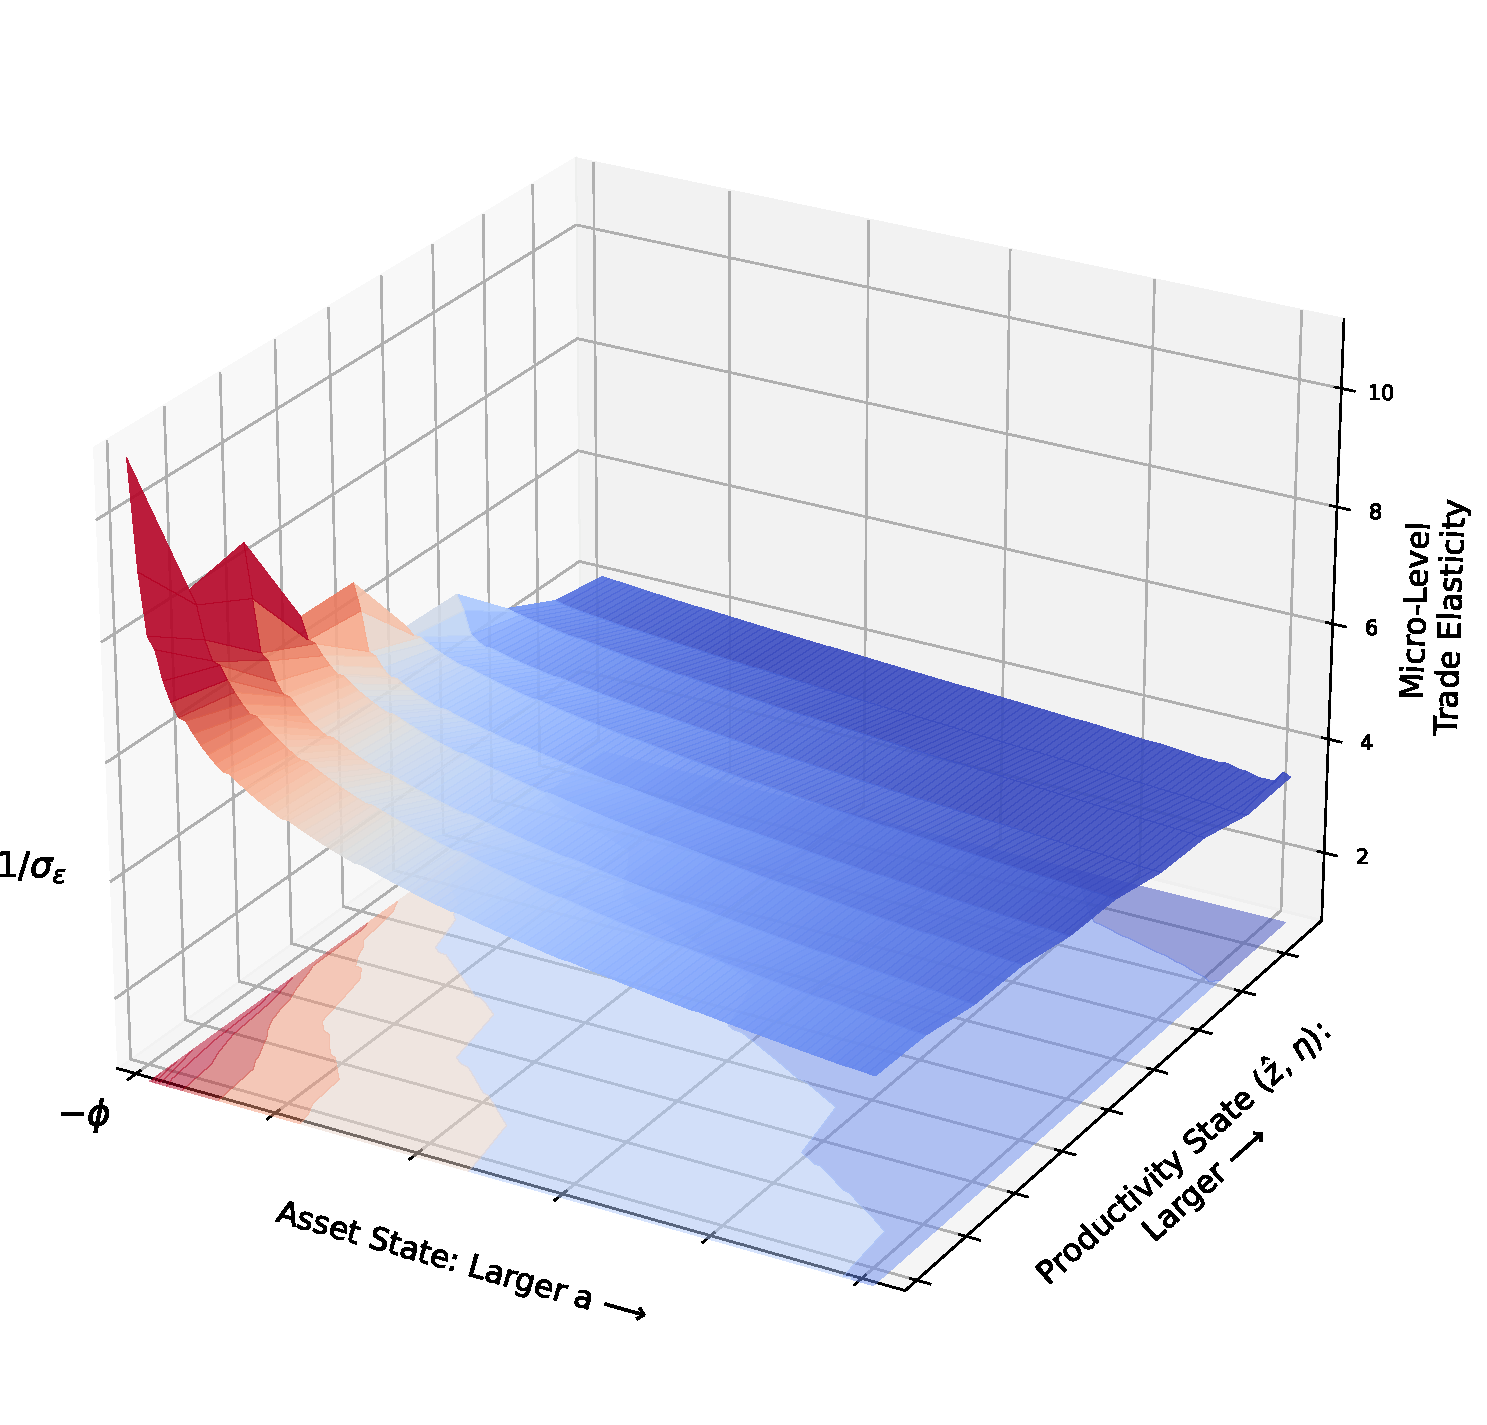
\includegraphics[scale = 0.45]{../notes/figures/micro-elasticity.pdf}}
\end{figure}
\end{frame}

%%%%%%%%%%%%%%%%%%%%%%%%%%%%%%%%%%%%%%%%%%%%%%%%%%%%%%%%%%%%%%%%%%%%%%%%%%%%%%%%%%%%%%%%%%%%%%%%
%%%%%%%%%%%%%%%%%%%%%%%%%%%%%%%%%%%%%%%%%%%%%%%%%%%%%%%%%%%%%%%%%%%%%%%%%%%%%%%%%%%%%%%%%%%%%%%%

\begin{frame}[t]{HA Gains from Trade}
\vspace{-.25cm}
\smallskip
{\small
\begin{prp}[{\normalsize HA Gains from Trade} ] \label{prp:gains-trade} The welfare gains from trade are given by
{\footnotesize
\begin{align}
\frac{\mathrm{d} W_{i}}{\mathrm{d} d_{ij} / d_{ij}} = \int_{a}\int_{z}  \bigg \{ \frac{\mathrm{d} v_i(a, z)}{\mathrm{d} d_{ij} / d_{ij}}  + v_{i}(a,z) \frac{\mathrm{d} \lambda_{i}(a,z)/ \lambda_{i}(a,z)}{\mathrm{d} d_{ij} / d_{ij}}  \bigg \} \lambda_{i}(a,z).
\nonumber
\end{align}
}which reflects the change in household level gains and how the distribution of households changes. Household level gains are given by
{\footnotesize
\begin{align}
\nonumber
\frac{\mathrm{d} v_i(a, z)}{\mathrm{d} d_{ij} / d_{ij}} = \mathbb{E}_{z} \sum_{t = 0}^{\infty} \beta^{t} \bigg \{ \begin{alert}<2>{ A(a_{t},z_{t}) }\end{alert} + \begin{alert}<3>{B(a_{t},z_{t})}\end{alert} + \begin{alert}<4>{C(a_{t},z_{t})}\end{alert} \bigg \}
\end{align}
}\end{prp}
}
\only<2>{
\medskip
This term is what I call the ``gains from substitution'':
{\small \begin{align*}
A(a,z) = -\sigma_{\epsilon} \frac{\mathrm{d} \pi_{ii}(a,z) / \pi_{ii}(a,z)}{\mathrm{d}d_{ij} / d_{ij}}  \\
\\
\approx -\sigma_{\epsilon} \times \pi_{ij}(a,z) \times \bar{\theta}(a,z) ^E_{ij}
\end{align*}
}\\
\medskip
Where the last line says these gains from substitution are about (i) exposure ( {\small \citet{deaton1989rice}, \citet{borusyak2021distributional} }) and (ii) elasticities ({\small \citet*{auer2022unequal}}).
}
\only<3>{
\medskip
This term is what I call the ``gains from changes in factor prices'':
{\small \begin{align*}
 B(a,z) = u'(c_{i}(a,z,i)) \times  a \times \frac{\mathrm{d} R_{i} / w_{i}}{\mathrm{d} d_{ij} / d_{ij}}
\end{align*}
}\\
\bigskip
How hh's real wealth ($+$ or $-$) change through GE effects on prices | all evaluated at the hh's marginal utility of home consumption.
}
\only<4>{
\medskip
This term is what I call the ``gains from changes in asset holdings''
\vspace{.15cm}
{\small
\begin{align*}
C(a,z) = \bigg \{\underbrace{ - \frac{u'(c_{i}(a,z,i))}{p_{ii}} + \beta \mathbb{E}_{z'} \bigg [-\sigma_{\epsilon} \frac{\partial \pi_{ii}(a',z') / \pi_{ii}(a',z')}{\partial a'} + \frac{u'(c_{i}(a',z',i))R_{i}}{p_{ii}} \bigg ] }_{\mbox{Euler equation}} \  \bigg \}\frac{\mathrm{d} g_{i}(a',z',i)}{\mathrm{d} d_{ij} / d_{ij}}
\end{align*}
}
\\
\medskip
which is zero for small changes as hh's are either (i) on their Euler equation or (ii) constrained and can't adjust their asset position.
}
\end{frame}


\begin{frame}[t]{HA Gains from Trade: $\log$ Preferences $\Rightarrow$ Separation of Trade and Heterogeneity}
\vspace{-.25cm}
\smallskip
{\small
\begin{prp}[{\normalsize Separation of Trade and Micro-Heterogeneity} ] In the heterogenous agent trade model where preferences are logarithmic over the physical commodity, the trade elasticity is
\begin{align}
\theta = -\frac{1}{\sigma_{\epsilon}}, \nonumber
\end{align}
and trade flows satisfy a standard gravity relationship
\begin{align}
\frac{M_{ij}}{M_{ii}} = \left( \frac{  w_{j} / A_{j} }{  w_{i} / A_{i} } \right)^{\frac{-1}{\sigma_{\epsilon}}} d_{ij}^{\frac{-1}{\sigma_{\epsilon}}}, \nonumber
\end{align}
and both are independent of the household heterogeneity. \uncover<2->{And the welfare gains from trade for an individual household are
\begin{align}
\nonumber
\frac{\mathrm{d} v_i(a, z)}{\mathrm{d} d_{ij} / d_{ij}} = \frac{1}{\theta (1-\beta)} \times \frac{\mathrm{d} \pi_{ii} / \pi_{ii}}{\mathrm{d}d_{ij} / d_{ij}} \ \ + \ \
\mathbb{E}_{z} \sum_{t = 0}^{\infty} \beta^{t} \bigg \{ B(a_{t},z_{t}) + C(a_{t},z_{t}) \bigg \}.
\end{align}
}
\end{prp}
}
\medskip
\only<1>{This mimics the results of \citet*{anderson1987ces}. This was not obvious to me given the environment \ldots risk, market incompleteness, borrowing constraints, etc.}
\only<2>{And we are back to \citet{arkolakis2012new} $+$ what's going on with factor prices and borrowing constraints.}
\end{frame}

%%%%%%%%%%%%%%%%%%%%%%%%%%%%%%%%%%%%%%%%%%%%%%%%%%%%%%%%%%%%%%%%%%%%%%%%%%%%%%%%%%%%%%%%%%%%%%%%
%%%%%%%%%%%%%%%%%%%%%%%%%%%%%%%%%%%%%%%%%%%%%%%%%%%%%%%%%%%%%%%%%%%%%%%%%%%%%%%%%%%%%%%%%%%%%%%%

\begin{frame}[t]{HA Gains from Trade under Efficiency}
\vspace{-.25cm}
\smallskip
{\small
\begin{prp}[{\normalsize Trade Elasticities and Welfare Gains in the Efficient Allocation}]\label{prp:gains-efficient-allocation} The elasticity of trade to a change in trade costs between $ij$ in the efficient allocation is:
\begin{align*}
\theta_{ij} =  -\frac{1}{\sigma_{\epsilon}} \bigg [ u'(c_{i}(j)) c_{i}(j) \bigg].
\end{align*}
\uncover<2->{And the welfare gains from a reduction in trade costs between $i,j$ are
\begin{align*}
\frac{\mathrm{d} W }{\mathrm{d} d_{ij} / d_{ij}} &= \frac{\sigma_{\epsilon} \  \theta_{ij} \  \pi_{ij} \ L_i}{1-\beta},
\end{align*}
which is the discounted, direct effect from relaxing the aggregate resource constraint.} \uncover<3->{And this can be expressed as
\begin{align*}
= -\sigma_{\epsilon} \times \frac{\mathrm{d} \pi_{ii} / \pi_{ii}}{\mathrm{d} d_{ij} / d_{ij}} \times \frac{L_i}{1 - \beta}.
\end{align*}}
\end{prp}
}
\medskip
\only<1>{Same idea as in decentralized allocation, but now everyone substitutes in a common way...}

\only<2>{Mimics the results of \citet{AtkesonBurstein2010} but with household (not firm) heterogeneity.}

\only<3>{And | again| we are back to an \citet{arkolakis2012new}-like expression and with $\log$ its exact.}
\end{frame}

%%%%%%%%%%%%%%%%%%%%%%%%%%%%%%%%%%%%%%%%%%%%%%%%%%%%%%%%%%%%%%%%%%%%%%%%%%%%%%%%%%%%%%%%%%%%%%%%
%%%%%%%%%%%%%%%%%%%%%%%%%%%%%%%%%%%%%%%%%%%%%%%%%%%%%%%%%%%%%%%%%%%%%%%%%%%%%%%%%%%%%%%%%%%%%%%%

\begin{frame}[t]{Quantitative Analysis}
\smallskip
\smallskip
This is what I'll do\ldots\\
\bigskip
\textbf{1.} Calibrate my model using my ``gravity as a guide'' approach on the 19 country data set of \citet{eaton2002technology} and targeting micro-evidence from \citet{borusyak2021distributional} and \citet{auer2022unequal}. \\
\bigskip
\textbf{2.} Gains from trade calculations.\\
\end{frame}

%%%%%%%%%%%%%%%%%%%%%%%%%%%%%%%%%%%%%%%%%%%%%%%%%%%%%%%%%%%%%%%%%%%%%%%%%%%%%%%%%%%%%%%%%%%%%%%%
%%%%%%%%%%%%%%%%%%%%%%%%%%%%%%%%%%%%%%%%%%%%%%%%%%%%%%%%%%%%%%%%%%%%%%%%%%%%%%%%%%%%%%%%%%%%%%%%

\begin{frame}[t]{Household Parameters}
\smallskip
Parameters common across countries:
\begin{itemize}
\smallskip
\item CRRA for $u$ with relative risk aversion $\gamma$ \uncover<2->{| varied to fit elasticities in \citet{auer2022unequal}}. \\
\smallskip
\item Earnings process as in \citet*{krueger2016macroeconomics}.
\smallskip
\item Discount factor $\beta$ jiggled to target a world interest rate of $1.0 \%$ in financial globalization case.
\end{itemize}
\bigskip
Parameters scaled across countries to deliver balanced-growth-like properties.
\begin{itemize}
\smallskip
\item Set $\sigma_{\epsilon,i} = \sigma_{\epsilon}\times A_i^{1-\gamma}$, \uncover<2->{| $\sigma_{\epsilon}$ varied to fit elasticities in \citet{auer2022unequal}}.
\medskip
\item Set the borrowing constraint so $\phi_{i} = \phi \times A_i$ where $\phi = 0.50$.
\end{itemize}
\bigskip
Household-specific quality shifters | a home bias term $\psi_{ii}(z)$ which additively shifts utility
\begin{itemize}
\smallskip
\item Without this prices and price elasticities determine shares, so to fit the data interactions between quality and household characteristics is a way; same idea as in \citet{berry1995automobile}.
\smallskip
\uncover<2->{\item Slope of $\psi_{ii}(z)$ wrt $z$ varied to fit \citet{borusyak2021distributional} facts.}
\end{itemize}
\end{frame}

%%%%%%%%%%%%%%%%%%%%%%%%%%%%%%%%%%%%%%%%%%%%%%%%%%%%%%%%%%%%%%%%%%%%%%%%%%%%%%%%%%%%%%%%%%%%%%%%
%%%%%%%%%%%%%%%%%%%%%%%%%%%%%%%%%%%%%%%%%%%%%%%%%%%%%%%%%%%%%%%%%%%%%%%%%%%%%%%%%%%%%%%%%%%%%%%%

\begin{frame}[t]{County Specific Parameters | Using Gravity as a Guide}
\smallskip
\only<1>{
The problem: no closed form map from trade flows to parameters as in standard trade models. But I want the model to replicate the geographic pattern of activity seen in the data.}
\only<2>{The solution: use the gravity regression ``as a guide'' where I estimate parameters of the model so that the regression coefficients run on my model's data match that seen in the data.}
\medskip
\uncover<2->{
\begin{itemize}
\smallskip
\item Step 0. Impose a trade cost function to reduce the parameter space
\begin{align}
\log d_{ij} = d_{k} + b + l + e_{h} + m_{i}. \nonumber
\end{align}
\smallskip
\item Step 1. Run this gravity regression on the data
\begin{align}
\log \left( {\frac{M_{ij}}{M_{ii}}} \right) = {Im_{i}} + {Ex_{j}} + {d_{k}} + {b} + {l} + {e_{h}} + \delta_{ij}. \nonumber
\end{align}
\smallskip
\item Step 2. Guess TFP terms and coefficients on the trade cost function, compute an equilibrium, run the same regression from above on model generated data.
\smallskip
\item Step 3. Evaluate difference between model and data and update parameters until convergence.
\end{itemize}
}
\end{frame}

%%%%%%%%%%%%%%%%%%%%%%%%%%%%%%%%%%%%%%%%%%%%%%%%%%%%%%%%%%%%%%%%%%%%%%%%%%%%%%%%%%%%%%%%%%%%%%%%
%%%%%%%%%%%%%%%%%%%%%%%%%%%%%%%%%%%%%%%%%%%%%%%%%%%%%%%%%%%%%%%%%%%%%%%%%%%%%%%%%%%%%%%%%%%%%%%%


\begin{frame}[t]{Bilateral Trade: Model vs. Data}
\begin{figure}[!t]
\centering{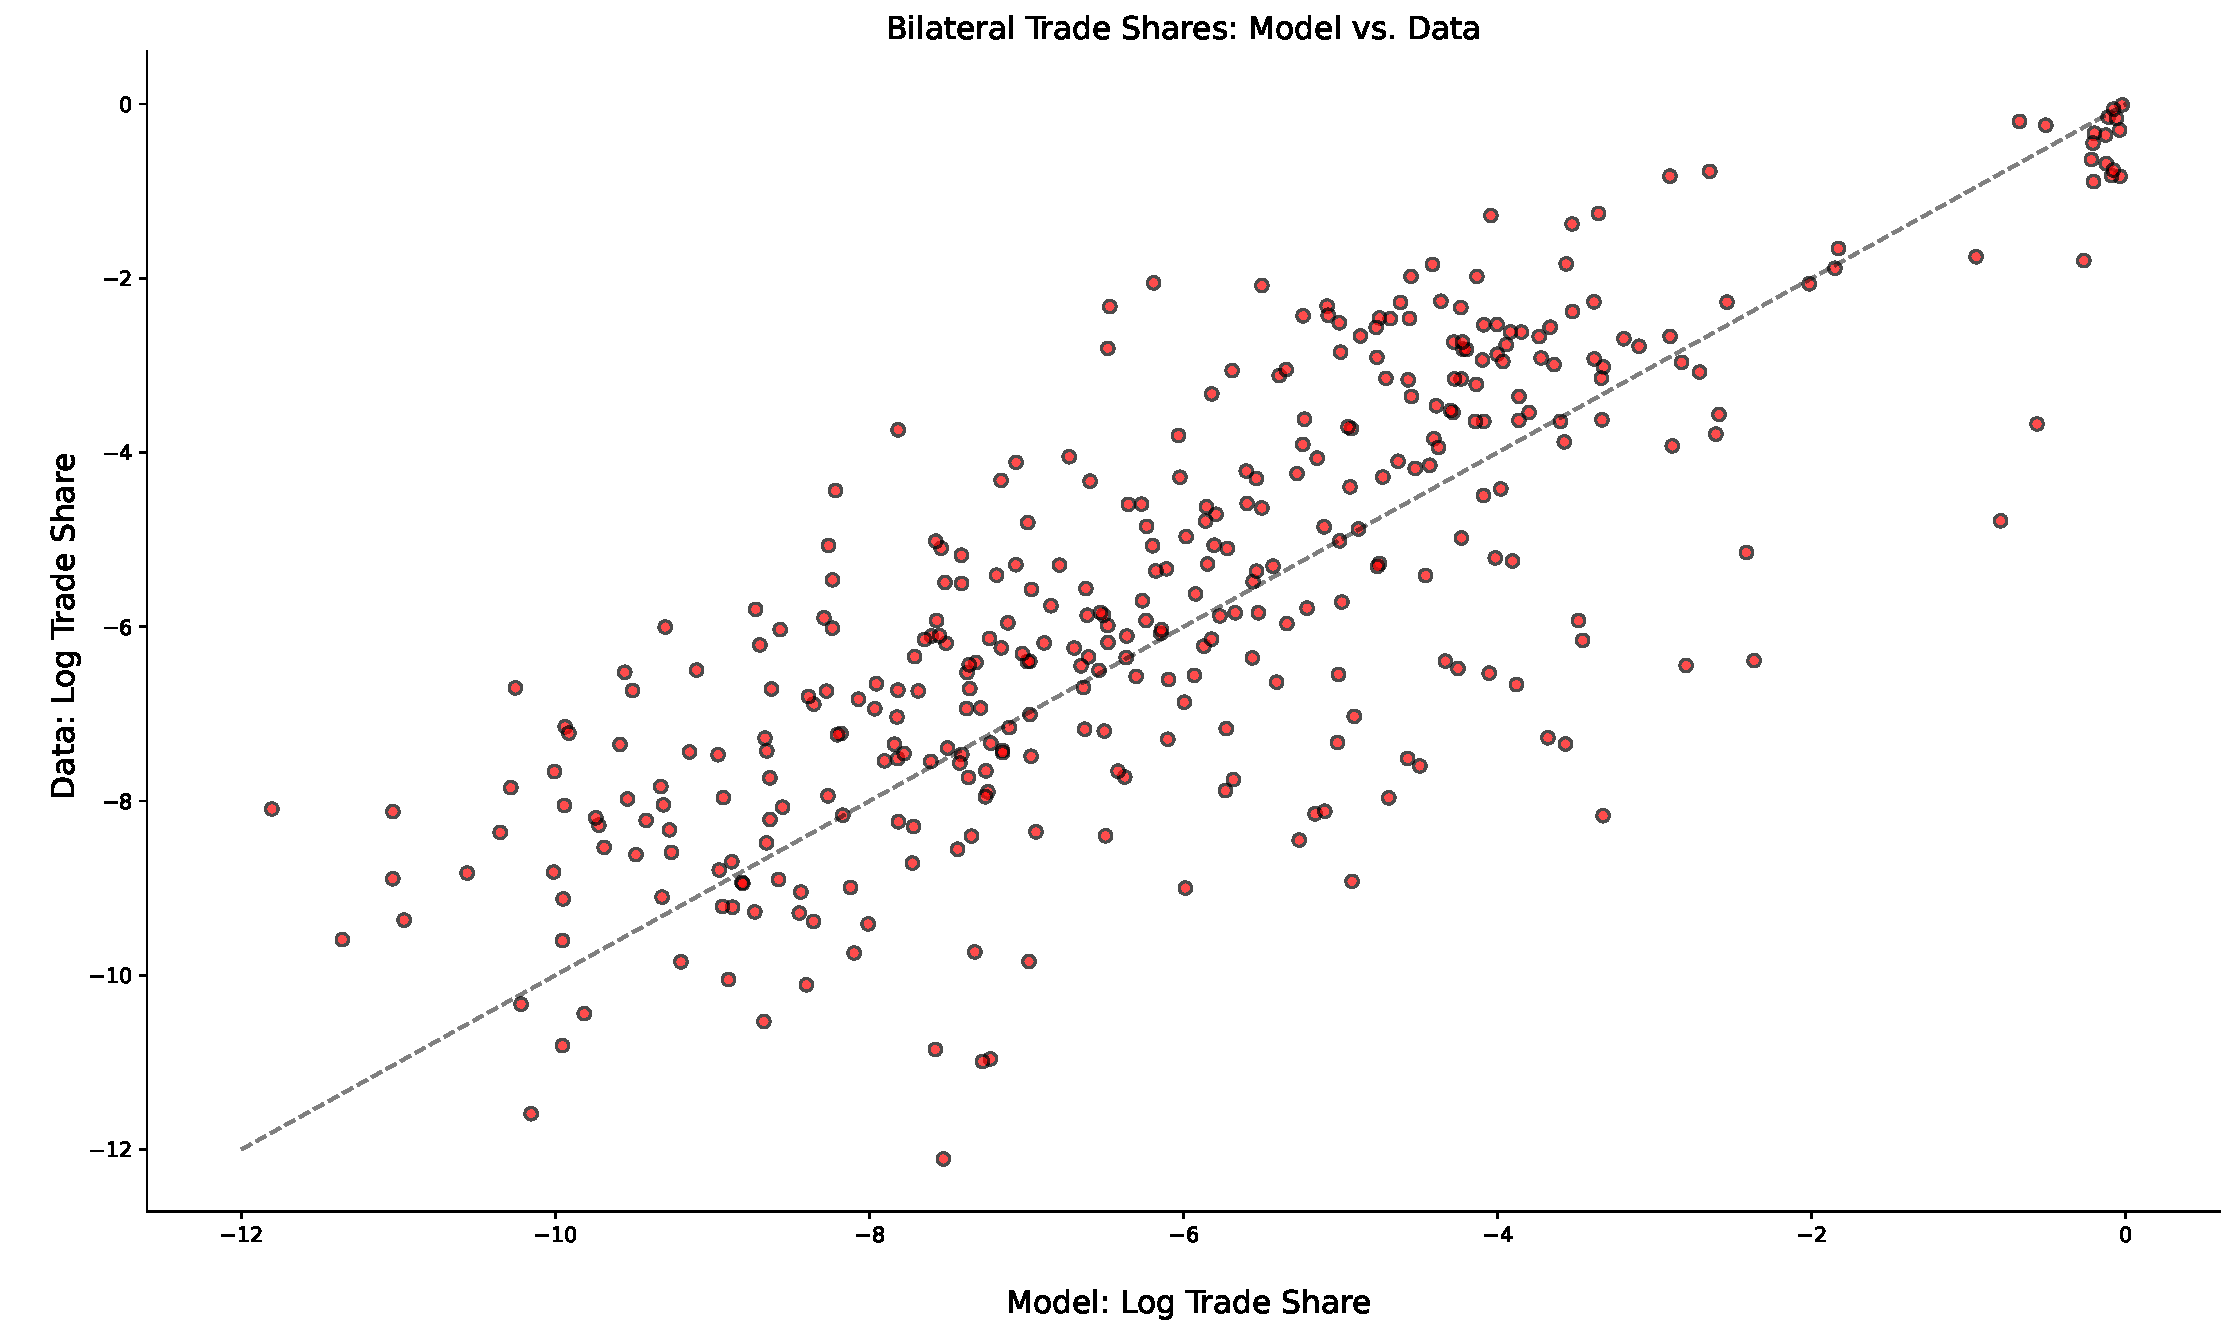
\includegraphics[scale = .35]{../notes/figures/trade-fit.pdf}}
\end{figure}
\end{frame}

%%%%%%%%%%%%%%%%%%%%%%%%%%%%%%%%%%%%%%%%%%%%%%%%%%%%%%%%%%%%%%%%%%%%%%%%%%%%%%%%%%%%%%%%%%%%%%%%
%%%%%%%%%%%%%%%%%%%%%%%%%%%%%%%%%%%%%%%%%%%%%%%%%%%%%%%%%%%%%%%%%%%%%%%%%%%%%%%%%%%%%%%%%%%%%%%%

\begin{frame}[t]
\frametitle{Estimates of Geographic Barriers}
\begin{table}[t]
\small
\begin{center}
\refstepcounter{table}
\setlength {\tabcolsep}{5.5mm}
\renewcommand{\arraystretch}{1.10}\label{tb-grav-est}
\begin{tabular}[t]{l c c c}
\multicolumn{4}{c}{{\normalsize\textbf{Table \ref{tb-grav-est}: Estimation Results}} }
\\\hline \hline
& & \multicolumn{2}{c}{\textbf{HAT-Model}}  \\
\cmidrule(lr){3-4}
Barrier& Moment & Model Fit & Parameter \\
\hline $[0,375)$                &$-3.10 $           & $-3.10 $              & $2.35$           \\
$[375,750)$                     &$-3.67 $           & $-3.67 $              & $2.81$           \\
$[750,1500)$                    &$-4.03 $           & $-4.03 $              & $3.09$           \\
$[1500,3000)$                   &$-4.22 $           & $-4.22 $              & $3.23$           \\
$[3000,6000)$                   &$-6.06 $           & $-6.06 $              & $4.88$           \\
$[6000,\mbox{maximum}]$         &$-6.56 $           & $-6.56 $              & $5.69$           \\
Shared border                   &$\phantom{-}0.30$  & $\phantom{-}0.30$     & $0.91$  \\
Language                        &$\phantom{-}0.51$  & $\phantom{-}0.51$     & $0.87$  \\
EFTA                            &$\phantom{-}0.04$  & $\phantom{-}0.04$     & $0.98$  \\
European Community              &$\phantom{-}0.54$  & $\phantom{-}0.54$     & $0.89$  \\
\hline
\end{tabular}
\\[0.5ex]
\parbox{4.2in}{\footnotesize \textbf{Note:} The first column reports data moments the HAT-model targets. The second reports the model moments. The third column reports the estimated parameter values.}
\end{center}
\end{table}
\bigskip
Far distances $\approx$ 10 percent less expensive than standard models would predict.
\end{frame}

%%%%%%%%%%%%%%%%%%%%%%%%%%%%%%%%%%%%%%%%%%%%%%%%%%%%%%%%%%%%%%%%%%%%%%%%%%%%%%%%%%%%%%%%%%%%%%%%
%%%%%%%%%%%%%%%%%%%%%%%%%%%%%%%%%%%%%%%%%%%%%%%%%%%%%%%%%%%%%%%%%%%%%%%%%%%%%%%%%%%%%%%%%%%%%%%%

\begin{frame}[t]{US Trade Elasticities: $-\theta_{us,j}$}
\begin{figure}[!t]
\centering{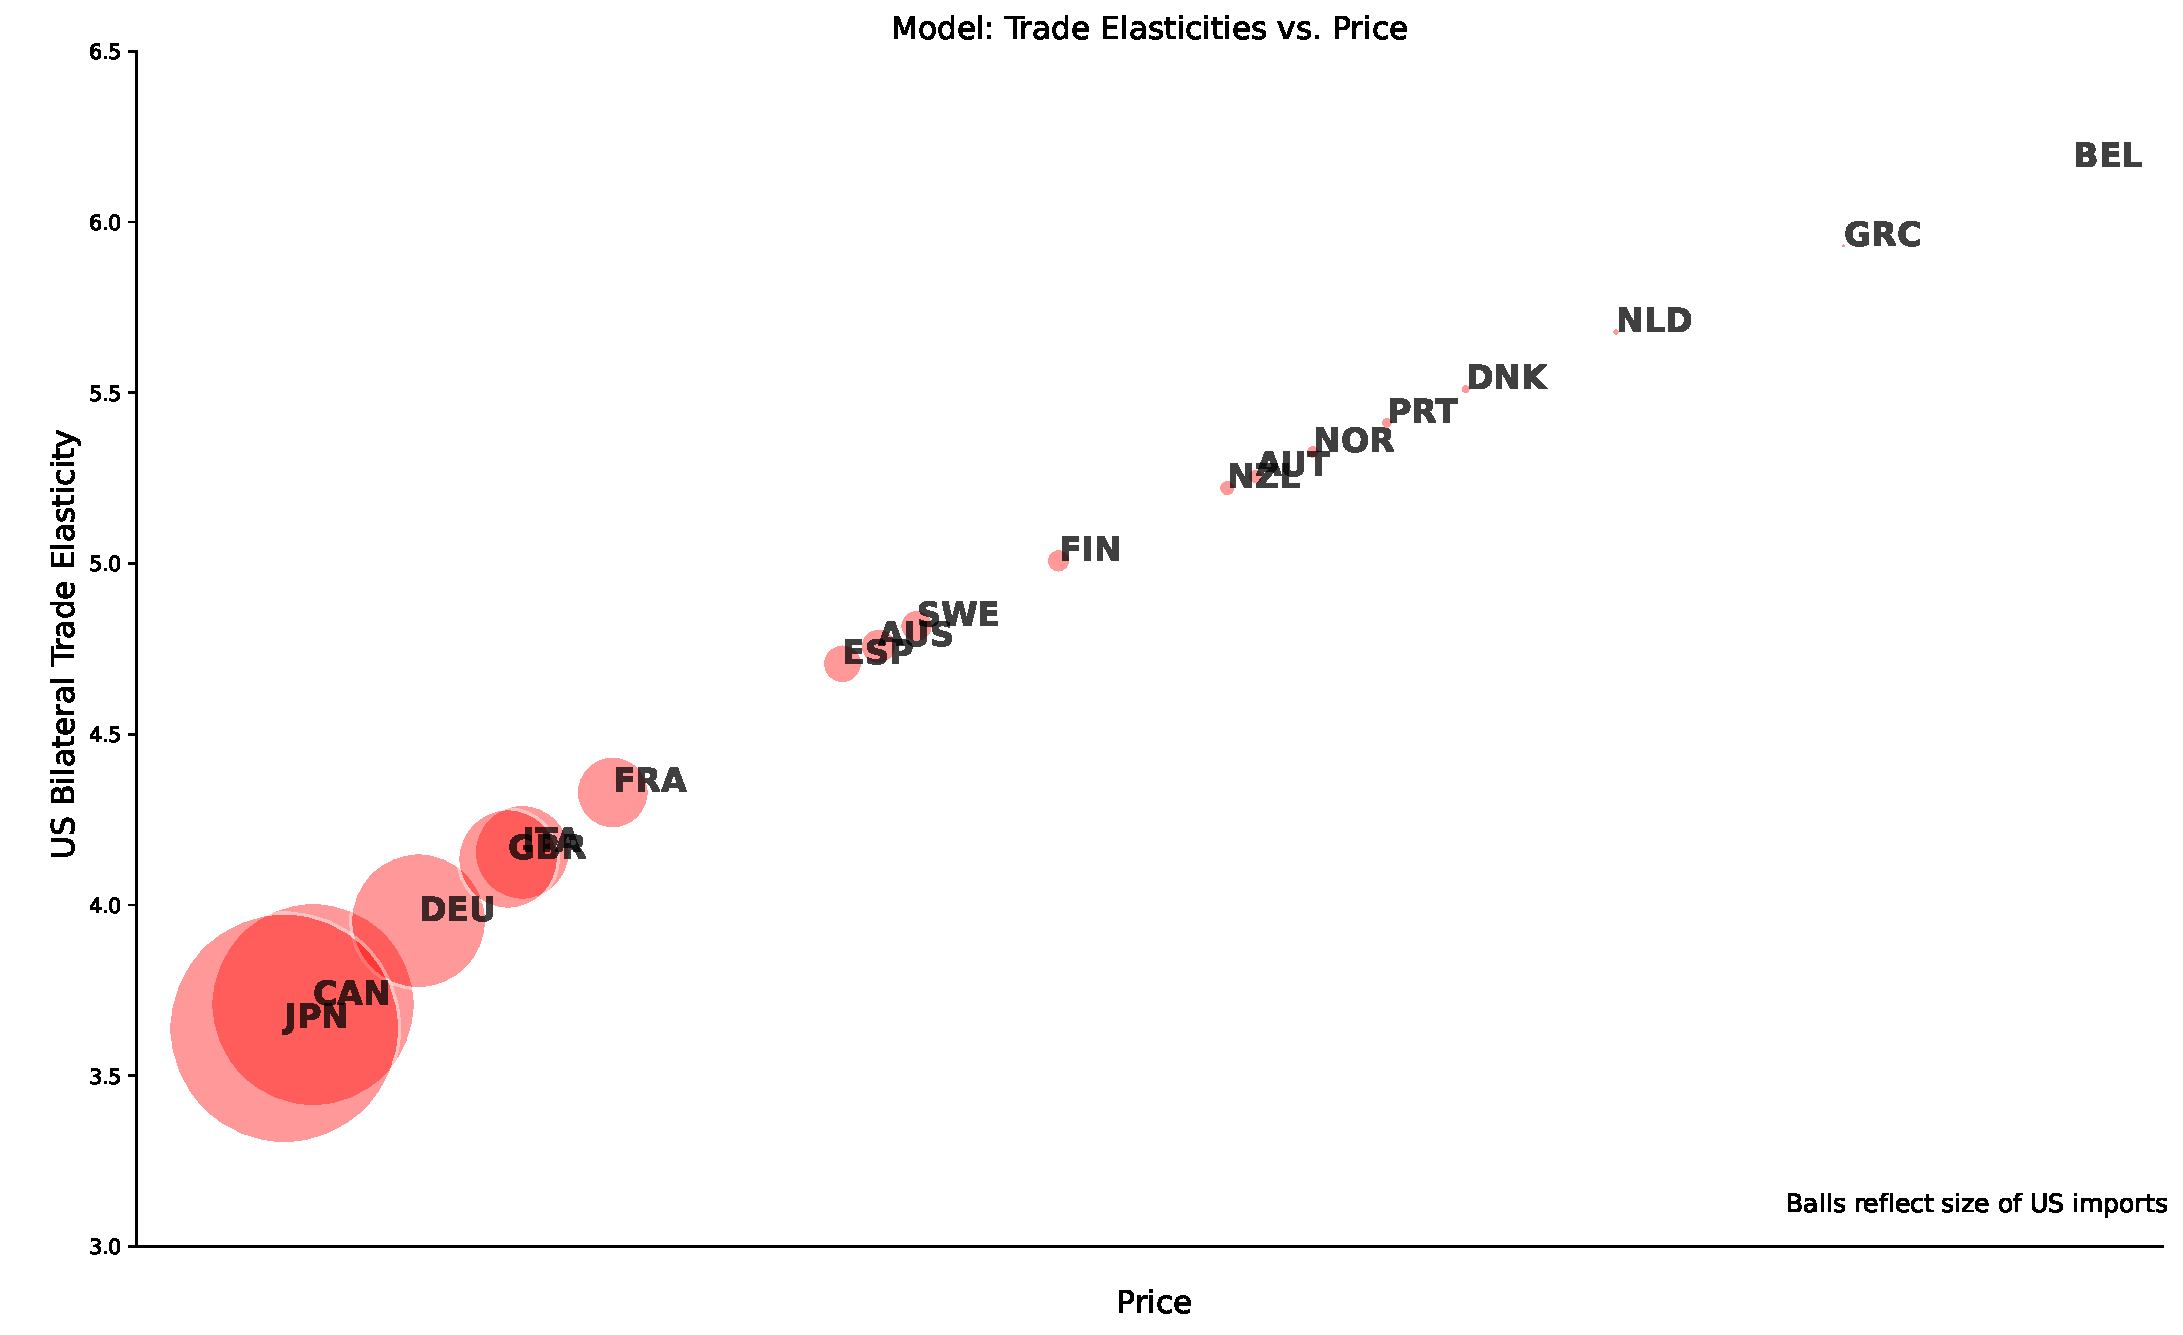
\includegraphics[scale = .33]{../notes/figures/us-elasticity.pdf}}
\end{figure}
\end{frame}

%%%%%%%%%%%%%%%%%%%%%%%%%%%%%%%%%%%%%%%%%%%%%%%%%%%%%%%%%%%%%%%%%%%%%%%%%%%%%%%%%%%%%%%%%%%%%%%%
%%%%%%%%%%%%%%%%%%%%%%%%%%%%%%%%%%%%%%%%%%%%%%%%%%%%%%%%%%%%%%%%%%%%%%%%%%%%%%%%%%%%%%%%%%%%%%%%
\begin{frame}[t]
\frametitle{Micro Moments | Model Consistent with Data}
\begin{table}[t]
\small
\begin{center}
\refstepcounter{table}
\setlength {\tabcolsep}{5.5mm}
\renewcommand{\arraystretch}{1.60}\label{tb-micro-shares}
\begin{tabular}[t]{l c c c}
\multicolumn{4}{c}{{\normalsize\textbf{Model: Shares, Elasticities, and MPCs by Income of US Households}} }
\\\hline \hline
& Import Shares & Trade Elasticities & MPCs\\
\cmidrule(lr){2-2} \cmidrule(lr){3-3} \cmidrule(lr){4-4}
Below Median Income & $0.08$ & $-6.64$ & 0.50\\
Median   & $0.08$ & $-4.48$ & 0.28\\
Above Median Income & $0.08$ & $-3.78$ & 0.17\\
\hline
\end{tabular}
\\[0.5ex]
%\parbox{5.95in}{\footnotesize \textbf{Note:} }
\end{center}
\end{table}
\bigskip
\begin{itemize}
\smallskip
\item Household-level import shares consistent with facts from  \citet{borusyak2021distributional}, i.e. rich and poor do not spend unequally on imports.
\smallskip
\item Household-level elasticities slightly understate those in \citet*{auer2022unequal}, rich more elastic than their estimates.
\smallskip
\item Household MPCs consistent with \citet{kaplan2022marginal}.
\end{itemize}
\end{frame}


\begin{frame}[t]
\frametitle{Measuring Welfare}
\smallskip
Want is a measure of welfare in interpretable units. No straight answer for a lot of reasons. \\
\medskip
I'm going to focus on equivalent variation.\\
\medskip
Reminder: Given some price change delivering utility level $V'$, equivalent variation asks ``at the old prices, $p_0$, how much extra income must be provided to be indifferent between $V'$ and $V(p_0)$?''\\
\bigskip
\bigskip
My measure is a permanent, proportional increase in income (asset and labor) $\tau_{i,a,z}$, at the old prices such that the new level of utility $v'_i$ is achieved:
\begin{align*}
v'_i(a, z ; \ p', R'_{i}, w'_{i}) - v_i(a, z ; \ p, \ R_{i}\tau_{i,a,z}, \ w_{i}\tau_{i,a,z})) = 0.
\end{align*}\\
\medskip
To be clear, this says a household with states $a,z$ must have their income increased today ( and for the infinite future ) by the number $\tau_{i,a,z}$.\\
\bigskip
Also, I'm doing this across steady states, not transitions. 
\end{frame}

%%%%%%%%%%%%%%%%%%%%%%%%%%%%%%%%%%%%%%%%%%%%%%%%%%%%%%%%%%%%%%%%%%%%%%%%%%%%%%%%%%%%%%%%%%%%%%%%
%%%%%%%%%%%%%%%%%%%%%%%%%%%%%%%%%%%%%%%%%%%%%%%%%%%%%%%%%%%%%%%%%%%%%%%%%%%%%%%%%%%%%%%%%%%%%%%

\begin{frame}[t]{U.S. Welfare: 10\% Reduction in $d_{us,j}$}
\begin{figure}[!t]
\centering{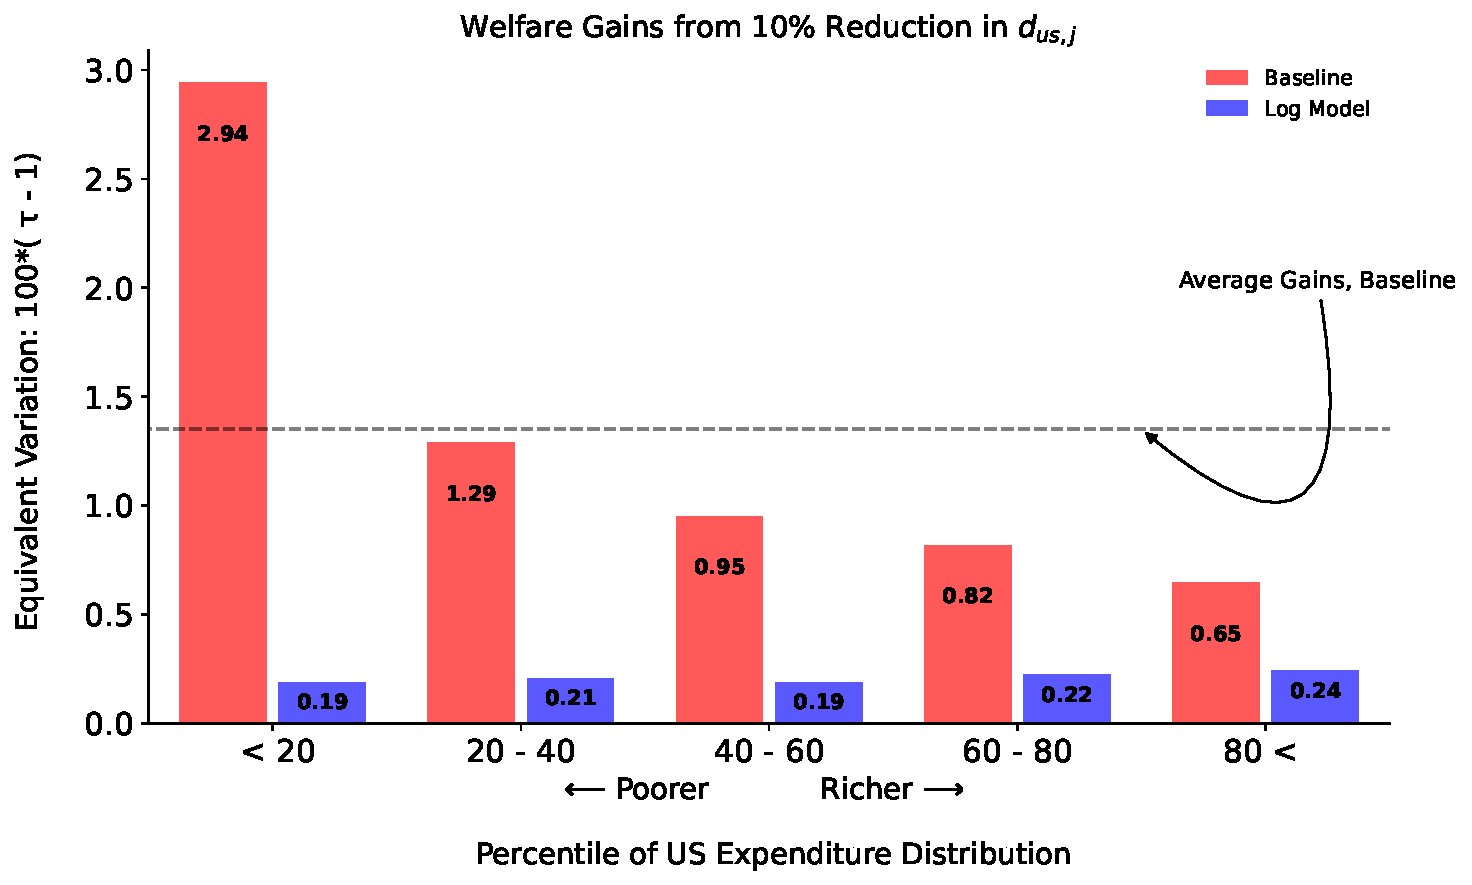
\includegraphics[scale = .55]{../notes/figures/ge-welfare-household-vs-log.pdf}}
\end{figure}
\end{frame}

%%%%%%%%%%%%%%%%%%%%%%%%%%%%%%%%%%%%%%%%%%%%%%%%%%%%%%%%%%%%%%%%%%%%%%%%%%%%%%%%%%%%%%%%%%%%%%%%
%%%%%%%%%%%%%%%%%%%%%%%%%%%%%%%%%%%%%%%%%%%%%%%%%%%%%%%%%%%%%%%%%%%%%%%%%%%%%%%%%%%%%%%%%%%%%%%

\begin{frame}[t]{U.S. Welfare: Global 10\% Reduction in $d$ }
\begin{figure}[!t]
\centering{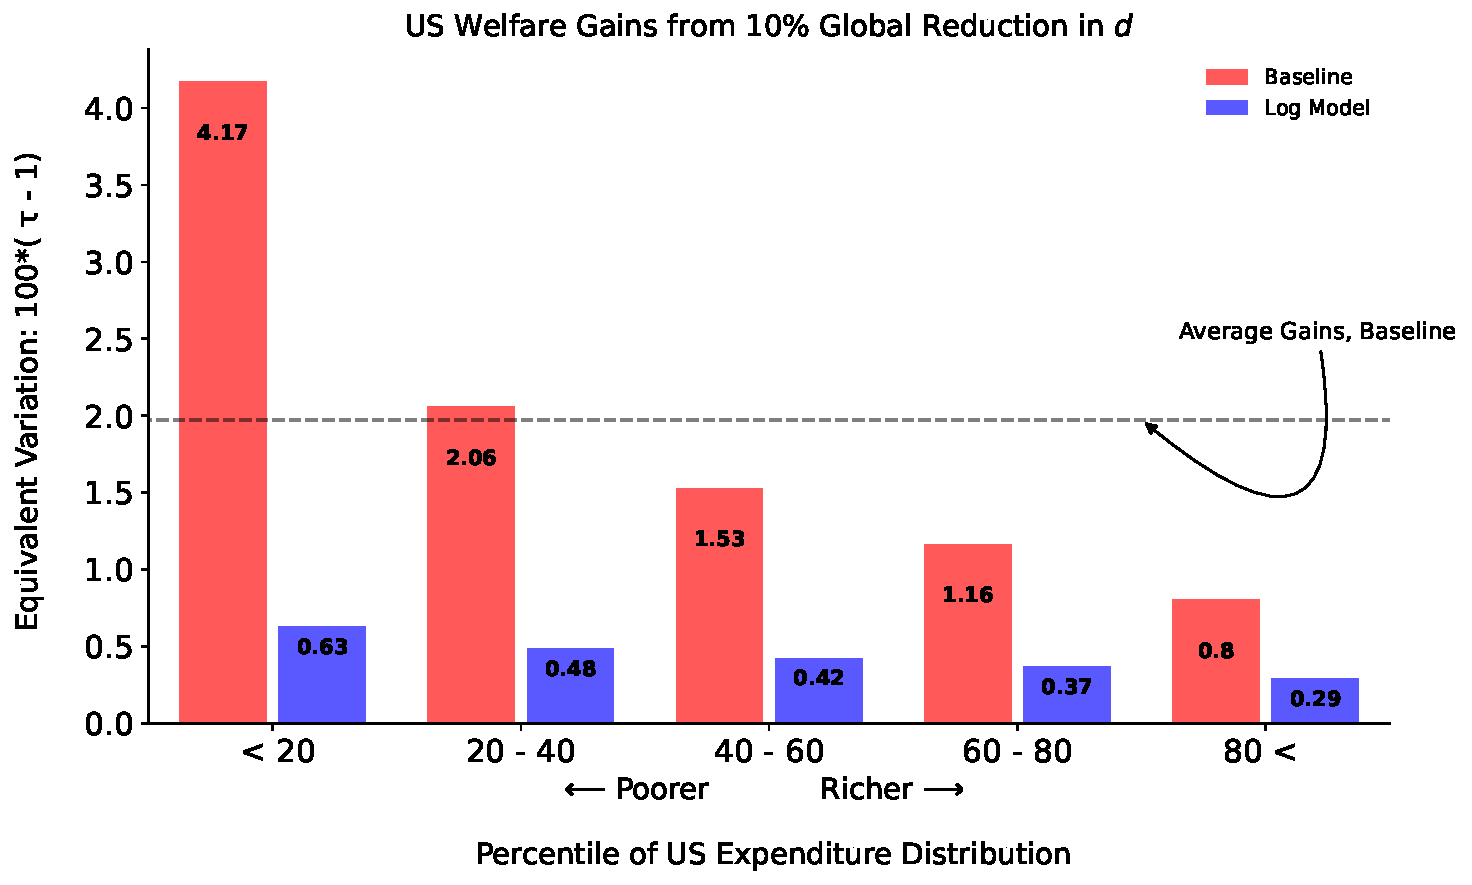
\includegraphics[scale = .55]{../notes/figures/global-welfare-household-vs-log.pdf}}
\end{figure}
\end{frame}


%%%%%%%%%%%%%%%%%%%%%%%%%%%%%%%%%%%%%%%%%%%%%%%%%%%%%%%%%%%%%%%%%%%%%%%%%%%%%%%%%%%%%%%%%%%%%%%%
%%%%%%%%%%%%%%%%%%%%%%%%%%%%%%%%%%%%%%%%%%%%%%%%%%%%%%%%%%%%%%%%%%%%%%%%%%%%%%%%%%%%%%%%%%%%%%%%

\begin{frame}[t]
\frametitle{Final Thoughts\ldots}
\smallskip
This paper has prompted even more questions\ldots
\begin{itemize}
\smallskip
\item The efficient pattern of trade? In a companion paper, I show that near-shoring is an outcome that a global planner likes.
\smallskip
\item Can trade policy improve outcomes? Put in tariffs and redistribute.
\smallskip
\item The interaction between trade goods and trade in assets?
\end{itemize}
\medskip
\bigskip
One more thing: My github repository provides the code and supplementary work behind this paper at \url{https://github.com/mwaugh0328/heterogeneous-agent-trade}.

\end{frame}

%%%%%%%%%%%%%%%%%%%%%%%%%%%%%%%%%%%%%%%%%%%%%%%%%%%%%%%%%%%%%%%%%%%%%%%%%%%%%%%%%%%%%%%%%%%%%%%%
%%%%%%%%%%%%%%%%%%%%%%%%%%%%%%%%%%%%%%%%%%%%%%%%%%%%%%%%%%%%%%%%%%%%%%%%%%%%%%%%%%%%%%%%%%%%%%%%

%%%%%%%%%%%%%%%%%%%%%%%%%%%%%%%%%%%%%%%%%%%%%%%%%%%%%%%%%%%%%%%%%%%%%%%%%%%%%%%%%%%%%%%%%%%%%%%%
%%%%%%%%%%%%%%%%%%%%%%%%%%%%%%%%%%%%%%%%%%%%%%%%%%%%%%%%%%%%%%%%%%%%%%%%%%%%%%%%%%%%%%%%%%%%%%%%

\appendix

\newcounter{finalframe}
\setcounter{finalframe}{\value{framenumber}}

\begin{frame}[allowframebreaks]
\frametitle{References}
\scriptsize
\bibliography{../notes/bibtex/micro_price_bibtex}
\end{frame}


\begin{frame}[t]{Log Model | Fit of Trade Data}
\begin{figure}[!t]
\centering{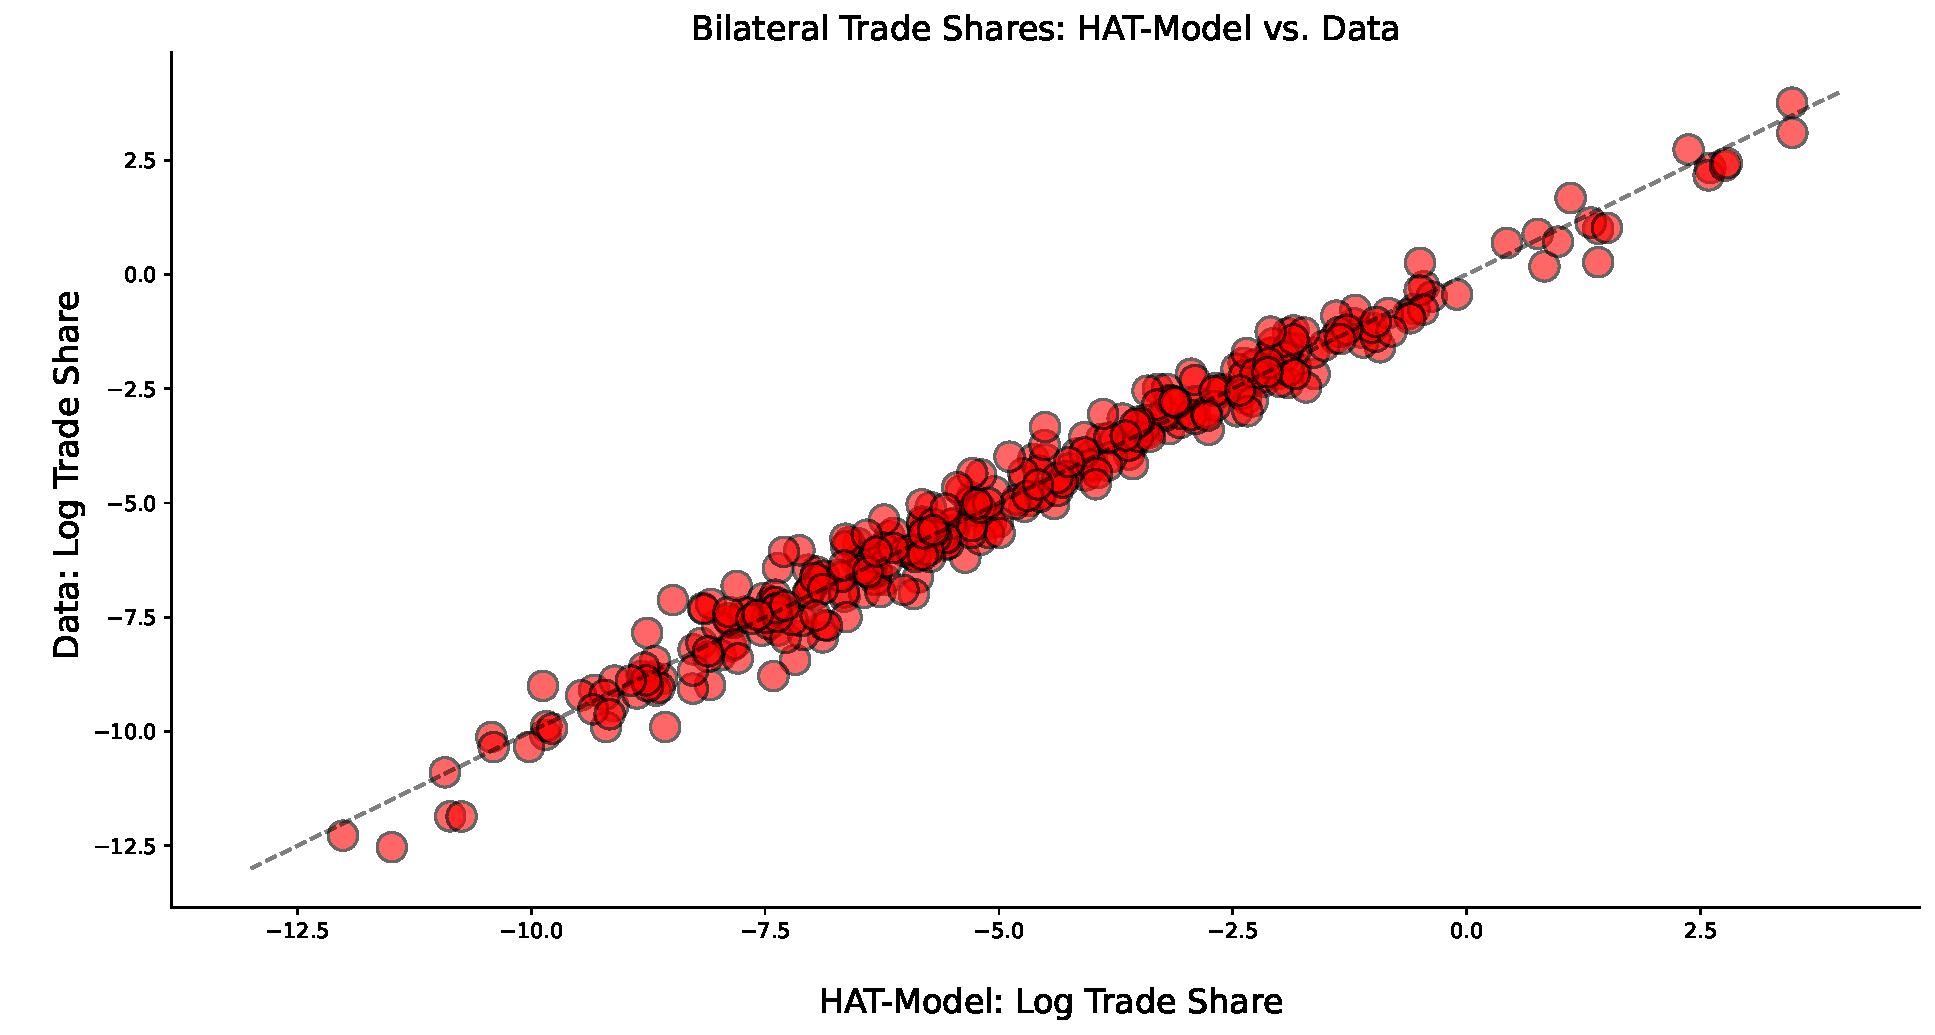
\includegraphics[scale = .35]{../notes/figures/log-trade-fit.pdf}}
\end{figure}
\end{frame}


%%%%%%%%%%%%%%%%%%%%%%%%%%%%%%%%%%%%%%%%%%%%%%%%%%%%%%%%%%%%%%%%%%%%%%%%%%%%%%%%%%%%%%%%%%%%%%%%
%%%%%%%%%%%%%%%%%%%%%%%%%%%%%%%%%%%%%%%%%%%%%%%%%%%%%%%%%%%%%%%%%%%%%%%%%%%%%%%%%%%%%%%%%%%%%%%%


\setcounter{framenumber}{\value{finalframe}}

%%%%%%%%%%%%%%%%%%%%%%%%%%%%%%%%%%%%%%%%%%%%%%%%%%%%%%%%%%%%%%%%%%%%%%%%%%%%%%%%%%%%%%%%%%%%%%%%%
%%%%%%%%%%%%%%%%%%%%%%%%%%%%%%%%%%%%%%%%%%%%%%%%%%%%%%%%%%%%%%%%%%%%%%%%%%%%%%%%%%%%%%%%%%%%%%%%%



\end{document} 